% Options for packages loaded elsewhere
\PassOptionsToPackage{unicode}{hyperref}
\PassOptionsToPackage{hyphens}{url}
%
\documentclass[
]{article}
\usepackage{lmodern}
\usepackage{amssymb,amsmath}
\usepackage{ifxetex,ifluatex}
\ifnum 0\ifxetex 1\fi\ifluatex 1\fi=0 % if pdftex
  \usepackage[T1]{fontenc}
  \usepackage[utf8]{inputenc}
  \usepackage{textcomp} % provide euro and other symbols
\else % if luatex or xetex
  \usepackage{unicode-math}
  \defaultfontfeatures{Scale=MatchLowercase}
  \defaultfontfeatures[\rmfamily]{Ligatures=TeX,Scale=1}
\fi
% Use upquote if available, for straight quotes in verbatim environments
\IfFileExists{upquote.sty}{\usepackage{upquote}}{}
\IfFileExists{microtype.sty}{% use microtype if available
  \usepackage[]{microtype}
  \UseMicrotypeSet[protrusion]{basicmath} % disable protrusion for tt fonts
}{}
\makeatletter
\@ifundefined{KOMAClassName}{% if non-KOMA class
  \IfFileExists{parskip.sty}{%
    \usepackage{parskip}
  }{% else
    \setlength{\parindent}{0pt}
    \setlength{\parskip}{6pt plus 2pt minus 1pt}}
}{% if KOMA class
  \KOMAoptions{parskip=half}}
\makeatother
\usepackage{xcolor}
\IfFileExists{xurl.sty}{\usepackage{xurl}}{} % add URL line breaks if available
\IfFileExists{bookmark.sty}{\usepackage{bookmark}}{\usepackage{hyperref}}
\hypersetup{
  pdftitle={``药物治疗是否影响癫痫次数?''-基于泊松回归模型的非正态的因变量(离散计数型数据)分析},
  pdfauthor={王昊(学号: 201821061107) 指导教师:段小刚},
  hidelinks,
  pdfcreator={LaTeX via pandoc}}
\urlstyle{same} % disable monospaced font for URLs
\usepackage[margin=1in]{geometry}
\usepackage{color}
\usepackage{fancyvrb}
\newcommand{\VerbBar}{|}
\newcommand{\VERB}{\Verb[commandchars=\\\{\}]}
\DefineVerbatimEnvironment{Highlighting}{Verbatim}{commandchars=\\\{\}}
% Add ',fontsize=\small' for more characters per line
\usepackage{framed}
\definecolor{shadecolor}{RGB}{248,248,248}
\newenvironment{Shaded}{\begin{snugshade}}{\end{snugshade}}
\newcommand{\AlertTok}[1]{\textcolor[rgb]{0.94,0.16,0.16}{#1}}
\newcommand{\AnnotationTok}[1]{\textcolor[rgb]{0.56,0.35,0.01}{\textbf{\textit{#1}}}}
\newcommand{\AttributeTok}[1]{\textcolor[rgb]{0.77,0.63,0.00}{#1}}
\newcommand{\BaseNTok}[1]{\textcolor[rgb]{0.00,0.00,0.81}{#1}}
\newcommand{\BuiltInTok}[1]{#1}
\newcommand{\CharTok}[1]{\textcolor[rgb]{0.31,0.60,0.02}{#1}}
\newcommand{\CommentTok}[1]{\textcolor[rgb]{0.56,0.35,0.01}{\textit{#1}}}
\newcommand{\CommentVarTok}[1]{\textcolor[rgb]{0.56,0.35,0.01}{\textbf{\textit{#1}}}}
\newcommand{\ConstantTok}[1]{\textcolor[rgb]{0.00,0.00,0.00}{#1}}
\newcommand{\ControlFlowTok}[1]{\textcolor[rgb]{0.13,0.29,0.53}{\textbf{#1}}}
\newcommand{\DataTypeTok}[1]{\textcolor[rgb]{0.13,0.29,0.53}{#1}}
\newcommand{\DecValTok}[1]{\textcolor[rgb]{0.00,0.00,0.81}{#1}}
\newcommand{\DocumentationTok}[1]{\textcolor[rgb]{0.56,0.35,0.01}{\textbf{\textit{#1}}}}
\newcommand{\ErrorTok}[1]{\textcolor[rgb]{0.64,0.00,0.00}{\textbf{#1}}}
\newcommand{\ExtensionTok}[1]{#1}
\newcommand{\FloatTok}[1]{\textcolor[rgb]{0.00,0.00,0.81}{#1}}
\newcommand{\FunctionTok}[1]{\textcolor[rgb]{0.00,0.00,0.00}{#1}}
\newcommand{\ImportTok}[1]{#1}
\newcommand{\InformationTok}[1]{\textcolor[rgb]{0.56,0.35,0.01}{\textbf{\textit{#1}}}}
\newcommand{\KeywordTok}[1]{\textcolor[rgb]{0.13,0.29,0.53}{\textbf{#1}}}
\newcommand{\NormalTok}[1]{#1}
\newcommand{\OperatorTok}[1]{\textcolor[rgb]{0.81,0.36,0.00}{\textbf{#1}}}
\newcommand{\OtherTok}[1]{\textcolor[rgb]{0.56,0.35,0.01}{#1}}
\newcommand{\PreprocessorTok}[1]{\textcolor[rgb]{0.56,0.35,0.01}{\textit{#1}}}
\newcommand{\RegionMarkerTok}[1]{#1}
\newcommand{\SpecialCharTok}[1]{\textcolor[rgb]{0.00,0.00,0.00}{#1}}
\newcommand{\SpecialStringTok}[1]{\textcolor[rgb]{0.31,0.60,0.02}{#1}}
\newcommand{\StringTok}[1]{\textcolor[rgb]{0.31,0.60,0.02}{#1}}
\newcommand{\VariableTok}[1]{\textcolor[rgb]{0.00,0.00,0.00}{#1}}
\newcommand{\VerbatimStringTok}[1]{\textcolor[rgb]{0.31,0.60,0.02}{#1}}
\newcommand{\WarningTok}[1]{\textcolor[rgb]{0.56,0.35,0.01}{\textbf{\textit{#1}}}}
\usepackage{graphicx,grffile}
\makeatletter
\def\maxwidth{\ifdim\Gin@nat@width>\linewidth\linewidth\else\Gin@nat@width\fi}
\def\maxheight{\ifdim\Gin@nat@height>\textheight\textheight\else\Gin@nat@height\fi}
\makeatother
% Scale images if necessary, so that they will not overflow the page
% margins by default, and it is still possible to overwrite the defaults
% using explicit options in \includegraphics[width, height, ...]{}
\setkeys{Gin}{width=\maxwidth,height=\maxheight,keepaspectratio}
% Set default figure placement to htbp
\makeatletter
\def\fps@figure{htbp}
\makeatother
\setlength{\emergencystretch}{3em} % prevent overfull lines
\providecommand{\tightlist}{%
  \setlength{\itemsep}{0pt}\setlength{\parskip}{0pt}}
\setcounter{secnumdepth}{5}
\usepackage{ctex}
% https://github.com/rstudio/rmarkdown/issues/337
\let\rmarkdownfootnote\footnote%
\def\footnote{\protect\rmarkdownfootnote}

% https://github.com/rstudio/rmarkdown/pull/252
\usepackage{titling}
\setlength{\droptitle}{-2em}

\pretitle{\vspace{\droptitle}\centering\huge}
\posttitle{\par}

\preauthor{\centering\large\emph}
\postauthor{\par}

\predate{\centering\large\emph}
\postdate{\par}

\title{``药物治疗是否影响癫痫次数?''-基于泊松回归模型的非正态的因变量(离散计数型数据)分析}
\author{王昊(学号: 201821061107) 指导教师:段小刚}
\date{2019年12月12日}

\begin{document}
\maketitle

{
\setcounter{tocdepth}{4}
\tableofcontents
}
\begin{center}\rule{0.5\linewidth}{\linethickness}\end{center}

\hypertarget{ux6458ux8981}{%
\section{摘要}\label{ux6458ux8981}}

本文探究了``八周中所发生的癫痫次数与药物治疗有何关系''的问题。我们使用广义线性模型分析非正态的因变量-离散的计数型数据,并探讨了对应的解决上述问题的模型:泊松回归模型,还包括拟合后参数的解释以及过度离势的判别和诊断,以及一些针对特殊情况的变种。

\hypertarget{ux80ccux666f}{%
\section{背景}\label{ux80ccux666f}}

\hypertarget{ux6570ux636eux6765ux6e90}{%
\subsection{数据来源}\label{ux6570ux636eux6765ux6e90}}

患有简单或复杂的部分性癫痫的患者被随机分为两组,一组服用抗癫痫药物氟柳双胺,另一组服用安慰剂。在连续四次的麻醉后门诊就诊中,每一次都报告了过去两周内癫痫发作的数量。

\hypertarget{ux5e7fux4e49ux7ebfux6027ux6a21ux578bux548cglmux51fdux6570}{%
\subsection{\texorpdfstring{广义线性模型和\texttt{glm()}函数}{广义线性模型和glm()函数}}\label{ux5e7fux4e49ux7ebfux6027ux6a21ux578bux548cglmux51fdux6570}}

\hypertarget{ux5e7fux4e49ux7ebfux6027ux6a21ux578b}{%
\subsubsection{广义线性模型}\label{ux5e7fux4e49ux7ebfux6027ux6a21ux578b}}

广义线性模型(Generalized linear model,
GLM)与标准线性模型的区别主要在于响应变量Y无需满足正态分布,只要服从指数分布族的一种分布即可,模型拟合的形式如下:
\[g\left(\mu_{Y}\right)=\beta_{0}+\sum_{j=1}^{p} \beta_{j} X_{j} \]
其中,\(g\left(\mu_{Y}\right)\)是条件均值的函数(称为连接函数),连接函数以及响应变量Y所满足的概率分布确定以后,广义线性模型通过最大似然估计(最大似然估计)的迭代推导出各个参数。

广义线性模型包含了非正态因变量的分析,其中,泊松回归(因变量为计数型)扩展了之前线性模型的框架。

\hypertarget{glmux51fdux6570}{%
\subsubsection{\texorpdfstring{\texttt{glm()}函数}{glm()函数}}\label{glmux51fdux6570}}

R中主要由\texttt{glm()}函数拟合广义线性模型,格式如下:

\begin{Shaded}
\begin{Highlighting}[]
\CommentTok{# glm(formula, family=family(link=function), data=)}
\end{Highlighting}
\end{Shaded}

以下举例说明\texttt{glm()}函数对泊松回归的拟合。

假设如下:

\begin{itemize}
\tightlist
\item
  响应变量:\(Y\)
\item
  三个预测变量:\(X_1,X_2,X_3\)
\item
  包含数据的数据框:mydata
\end{itemize}

泊松回归使用在给定时间内响应变量为事件发生数目的情形。

假设Y服从泊松分布,则线性模型的拟合形式为:
\[\log _{e}(\lambda)=\beta_{0}+\sum_{j=1}^{p} \beta_{j} X_{j}\]
其中\(\lambda\)是Y的均值,\(log(\lambda)\)为连接函数,概率分布为泊松分布,泊松回归模型拟合代码如下:

\begin{Shaded}
\begin{Highlighting}[]
\CommentTok{# glm(Y~X1+X2+X3, family=position(link="log"), data=mydata)}
\end{Highlighting}
\end{Shaded}

值得一提的是,如果令连接函数\(g\left(\mu_{Y}\right)=\mu_{Y}\),并设定概率分布为正态(高斯)分布,那么此时的线性回归模型拟合代码如下:

\begin{Shaded}
\begin{Highlighting}[]
\CommentTok{# glm(Y~X1+X2+X3, family=gaussian(link="identity"), data=mydata)}
\end{Highlighting}
\end{Shaded}

此时生成的结果与下列代码的结果相同:

\begin{Shaded}
\begin{Highlighting}[]
\CommentTok{#lm(Y~X1+X2+X3, data=mydata)}
\end{Highlighting}
\end{Shaded}

此时的\texttt{glm()}函数所模拟的广义线性模型与标准线性模型等价,也就是说,标准线性模型是广义线性模型的一种特例。

综上所述,广义线性模型不直接拟合响应变量Y本身的条件均值,而不是拟合响应变量Y的条件均值的一个函数,并假设响应变量服从指数分布族中的某个分布,采用极大似然估计而非最小二乘法为推到依据,极大地扩展了线性模型的适用范围。

\hypertarget{ux7814ux7a76ux95eeux9898}{%
\section{研究问题}\label{ux7814ux7a76ux95eeux9898}}

八周中所发生的癫痫次数与药物治疗有何关系。患有简单或复杂的部分性癫痫的患者被随机分为两组,一组服用抗癫痫药物progabide,另一组服用安慰剂。在连续四次的麻醉后门诊就诊中,每一次都报告了过去两周内癫痫发作的数量。我们研究的问题是:药物治疗是否影响癫痫次数?

\hypertarget{ux5bf9ux6570ux636eux7684ux63cfux8ff0ux6027ux5206ux6790}{%
\section{对数据的描述性分析}\label{ux5bf9ux6570ux636eux7684ux63cfux8ff0ux6027ux5206ux6790}}

Breslow数据的因变量为 sumY
(随机化后八周内癫痫发病数),预测变量为治疗条件(Trt
)、年龄(Age)和前八周内的基础癫痫发病数(base)。包含基础癫痫发病数和年龄的原因在于他们对响应变量有潜在影响。我们最终感兴趣的是药物治疗是否能减少癫痫发病数。

泊松回归通常用于通过一系列连续型和/或类别型预测变量来预测计数型结果变量。以下将采用\texttt{robust}包中的Breslow数据阐述泊松回归的应用。

\hypertarget{ux5b89ux88c5robustux5305}{%
\subsection{安装robust包:}\label{ux5b89ux88c5robustux5305}}

\begin{Shaded}
\begin{Highlighting}[]
\CommentTok{#install.packages("robust")}
\end{Highlighting}
\end{Shaded}

\hypertarget{ux67e5ux770bux6570ux636eux96c6ux7684ux7edfux8ba1ux6c47ux603bux4fe1ux606f}{%
\subsection{查看数据集的统计汇总信息:}\label{ux67e5ux770bux6570ux636eux96c6ux7684ux7edfux8ba1ux6c47ux603bux4fe1ux606f}}

\begin{Shaded}
\begin{Highlighting}[]
\KeywordTok{data}\NormalTok{(breslow.dat, }\DataTypeTok{package =} \StringTok{"robust"}\NormalTok{)}
\KeywordTok{names}\NormalTok{(breslow.dat)}
\end{Highlighting}
\end{Shaded}

\begin{verbatim}
##  [1] "ID"    "Y1"    "Y2"    "Y3"    "Y4"    "Base"  "Age"   "Trt"   "Ysum" 
## [10] "sumY"  "Age10" "Base4"
\end{verbatim}

\begin{Shaded}
\begin{Highlighting}[]
\KeywordTok{summary}\NormalTok{(breslow.dat[}\KeywordTok{c}\NormalTok{(}\DecValTok{6}\NormalTok{,}\DecValTok{7}\NormalTok{,}\DecValTok{8}\NormalTok{,}\DecValTok{10}\NormalTok{)])}
\end{Highlighting}
\end{Shaded}

\begin{verbatim}
##       Base             Age               Trt          sumY       
##  Min.   :  6.00   Min.   :18.00   placebo  :28   Min.   :  0.00  
##  1st Qu.: 12.00   1st Qu.:23.00   progabide:31   1st Qu.: 11.50  
##  Median : 22.00   Median :28.00                  Median : 16.00  
##  Mean   : 31.22   Mean   :28.34                  Mean   : 33.05  
##  3rd Qu.: 41.00   3rd Qu.:32.00                  3rd Qu.: 36.00  
##  Max.   :151.00   Max.   :42.00                  Max.   :302.00
\end{verbatim}

虽然数据集一共有12个变量,但是我们只关心之前描述的四个变量。对于因变量,我们用如下代码生成下列图形:

\begin{Shaded}
\begin{Highlighting}[]
\NormalTok{opar <-}\StringTok{ }\KeywordTok{par}\NormalTok{(}\DataTypeTok{no.readonly =} \OtherTok{TRUE}\NormalTok{)}
\KeywordTok{par}\NormalTok{(}\DataTypeTok{mfow=}\KeywordTok{c}\NormalTok{(}\DecValTok{1}\NormalTok{,}\DecValTok{2}\NormalTok{))}
\KeywordTok{attach}\NormalTok{(breslow.dat)}
\KeywordTok{hist}\NormalTok{(sumY, }\DataTypeTok{breaks =} \DecValTok{20}\NormalTok{, }
       \DataTypeTok{xlab =} \StringTok{"Seizure Count"}\NormalTok{,}
       \DataTypeTok{main =} \StringTok{"Distribution of Seizures"}\NormalTok{)}
\end{Highlighting}
\end{Shaded}

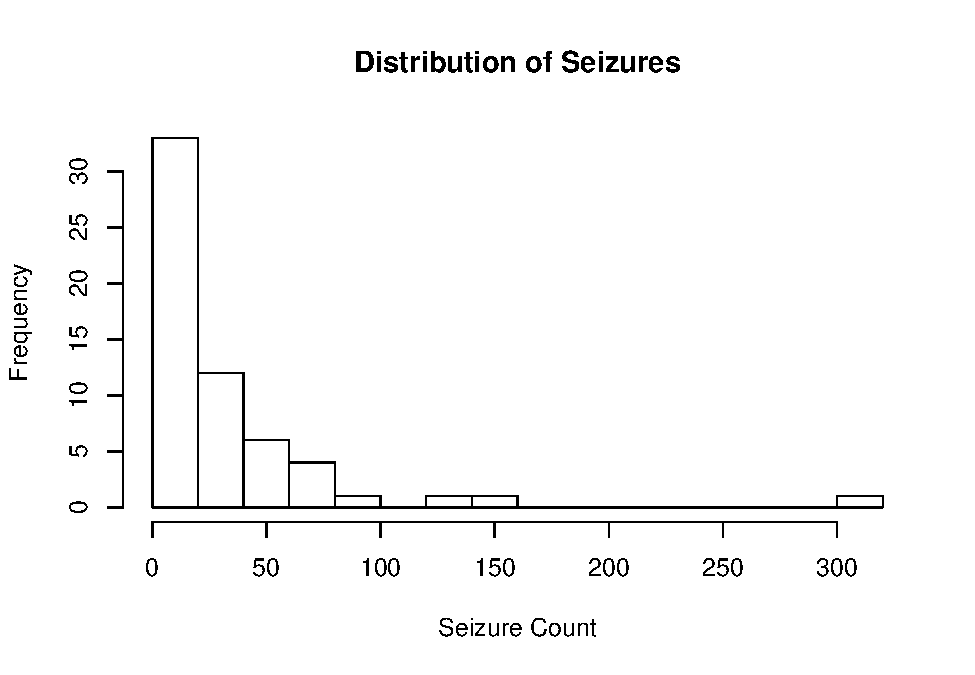
\includegraphics{R_Homework_2_201821061107_files/figure-latex/unnamed-chunk-7-1.pdf}

\begin{Shaded}
\begin{Highlighting}[]
\KeywordTok{boxplot}\NormalTok{(sumY}\OperatorTok{~}\NormalTok{Trt, }
        \DataTypeTok{xlab=}\StringTok{"Treatment"}\NormalTok{,}
        \DataTypeTok{main =} \StringTok{"Group Comparisons"}\NormalTok{)}
\end{Highlighting}
\end{Shaded}

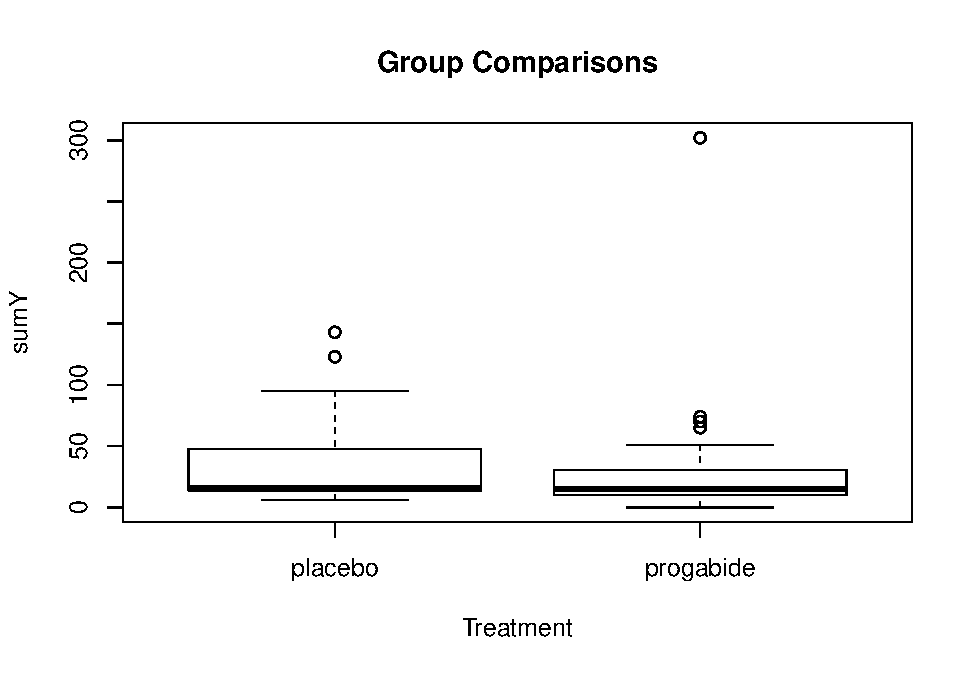
\includegraphics{R_Homework_2_201821061107_files/figure-latex/unnamed-chunk-8-1.pdf}

\begin{Shaded}
\begin{Highlighting}[]
\KeywordTok{par}\NormalTok{(opar)}
\end{Highlighting}
\end{Shaded}

上图清楚地展示了因变量的偏倚特性和可能存在的离群点,而且在药物治疗下癫痫发病数似乎变小了,且方差也变小了。

\hypertarget{ux7edfux8ba1ux6a21ux578bux7684ux5177ux4f53ux5f62ux5f0f}{%
\section{统计模型的具体形式}\label{ux7edfux8ba1ux6a21ux578bux7684ux5177ux4f53ux5f62ux5f0f}}

下面用泊松回归进行拟合:

\begin{Shaded}
\begin{Highlighting}[]
\NormalTok{fit <-}\StringTok{ }\KeywordTok{glm}\NormalTok{(sumY }\OperatorTok{~}\StringTok{ }\NormalTok{Base }\OperatorTok{+}\StringTok{ }\NormalTok{Age }\OperatorTok{+}\StringTok{ }\NormalTok{Trt, }\DataTypeTok{data =}\NormalTok{ breslow.dat, }
           \DataTypeTok{family =} \KeywordTok{poisson}\NormalTok{())}
\KeywordTok{summary}\NormalTok{(fit)}
\end{Highlighting}
\end{Shaded}

\begin{verbatim}
## 
## Call:
## glm(formula = sumY ~ Base + Age + Trt, family = poisson(), data = breslow.dat)
## 
## Deviance Residuals: 
##     Min       1Q   Median       3Q      Max  
## -6.0569  -2.0433  -0.9397   0.7929  11.0061  
## 
## Coefficients:
##                Estimate Std. Error z value Pr(>|z|)    
## (Intercept)   1.9488259  0.1356191  14.370  < 2e-16 ***
## Base          0.0226517  0.0005093  44.476  < 2e-16 ***
## Age           0.0227401  0.0040240   5.651 1.59e-08 ***
## Trtprogabide -0.1527009  0.0478051  -3.194   0.0014 ** 
## ---
## Signif. codes:  0 '***' 0.001 '**' 0.01 '*' 0.05 '.' 0.1 ' ' 1
## 
## (Dispersion parameter for poisson family taken to be 1)
## 
##     Null deviance: 2122.73  on 58  degrees of freedom
## Residual deviance:  559.44  on 55  degrees of freedom
## AIC: 850.71
## 
## Number of Fisher Scoring iterations: 5
\end{verbatim}

\hypertarget{ux6a21ux578bux7684ux7ed3ux679cux5206ux6790ux4e0eux89e3ux91ca}{%
\section{模型的结果分析与解释}\label{ux6a21ux578bux7684ux7ed3ux679cux5206ux6790ux4e0eux89e3ux91ca}}

\hypertarget{ux89e3ux91caux6a21ux578bux53c2ux6570}{%
\subsection{解释模型参数}\label{ux89e3ux91caux6a21ux578bux53c2ux6570}}

Logistic回归是对数优势比,在泊松回归中,因变量以条件均值的对数形式\(\log _{e}(\lambda)\)来建模,响应的初始模型参数为对数均值,同样也可以进行指数化以探求因变量的初始尺度上解释回归系数。以下代码给出了着两者的参数:

\begin{Shaded}
\begin{Highlighting}[]
\KeywordTok{coef}\NormalTok{(fit)}
\end{Highlighting}
\end{Shaded}

\begin{verbatim}
##  (Intercept)         Base          Age Trtprogabide 
##   1.94882593   0.02265174   0.02274013  -0.15270095
\end{verbatim}

\begin{Shaded}
\begin{Highlighting}[]
\KeywordTok{exp}\NormalTok{(}\KeywordTok{coef}\NormalTok{(fit))}
\end{Highlighting}
\end{Shaded}

\begin{verbatim}
##  (Intercept)         Base          Age Trtprogabide 
##    7.0204403    1.0229102    1.0230007    0.8583864
\end{verbatim}

\hypertarget{ux5e74ux9f84}{%
\subsubsection{年龄}\label{ux5e74ux9f84}}

年龄的回归参数为0.0227,表明保持其他预测变量不变,年龄增加一岁,癫痫发病数的对数均值将相应增加0.03。

\hypertarget{ux622aux8dddux9879}{%
\subsubsection{截距项}\label{ux622aux8dddux9879}}

截距项为预测变量都为0时,发病数的对数均值,显然年龄不可能为0,而且调查对象的基础发病数也都不为0,因此截距项没有实际意义。

\hypertarget{trtprogabide}{%
\subsubsection{Trtprogabide}\label{trtprogabide}}

从指数化的系数可以看出,保持其他变量不变,年龄增加一岁,期望的癫痫发病数将乘以1.023。这意味着年龄的增加与较高的癫痫发病数相关联。更为重要的是,一单位
Trt
的变化(即从安慰剂到治疗组),期望的癫痫发病数将乘以0.86,换句话说,保持基础癫痫发病数和年龄不变,服药组相对于安慰剂组癫痫发病数降低了20\%。

需要注意的是,与Logistic回归中的指数化参数相似,泊松模型中的指数化参数对响应变量的影响都是成倍增加的,而不是线性相加。

\hypertarget{ux8fc7ux5ea6ux79bbux52bf}{%
\subsection{过度离势}\label{ux8fc7ux5ea6ux79bbux52bf}}

泊松分布的期望和方差相等。当因变量观测的方差比依据泊松分布预测的方差大时,泊松回归可能发生过度离势。可能发生过度离势的原因有如下几个:

\begin{itemize}
\tightlist
\item
  遗漏了某个重要的预测变量;
\item
  可能因为事件相关,在在泊松分布的观测中,计数中每次事件都被认为是独立发生的;
\item
  在纵向数据分析中,重复测量的数据由于内在群聚特性可导致过度离势。
\end{itemize}

如果过度离势发生了,在模型中你无法进行解释,那么有可能你会发现并不真实存在的效应。

判断过度离势是否发生的准则依然是残差偏差与残差自由度的比例,如果远远大于1则表明存在过度离势。对于上述癫痫发病数数据,它的比例是:

\begin{Shaded}
\begin{Highlighting}[]
\KeywordTok{deviance}\NormalTok{(fit)}\OperatorTok{/}\KeywordTok{df.residual}\NormalTok{(fit)}
\end{Highlighting}
\end{Shaded}

\begin{verbatim}
## [1] 10.1717
\end{verbatim}

很显然,比例远大于1,存在过度离势。

qcc包提供了一个对泊松模型过度离势的检验方法。

\begin{Shaded}
\begin{Highlighting}[]
\CommentTok{#install.packages("qcc")}
\end{Highlighting}
\end{Shaded}

\begin{Shaded}
\begin{Highlighting}[]
\KeywordTok{library}\NormalTok{(qcc)}
\end{Highlighting}
\end{Shaded}

\begin{verbatim}
## Package 'qcc' version 2.7
\end{verbatim}

\begin{verbatim}
## Type 'citation("qcc")' for citing this R package in publications.
\end{verbatim}

\begin{Shaded}
\begin{Highlighting}[]
\KeywordTok{qcc.overdispersion.test}\NormalTok{(breslow.dat}\OperatorTok{$}\NormalTok{sumY, }
                        \DataTypeTok{type =} \StringTok{"poisson"}\NormalTok{)}\CommentTok{#检验}
\end{Highlighting}
\end{Shaded}

\begin{verbatim}
##                    
## Overdispersion test Obs.Var/Theor.Var Statistic p-value
##        poisson data          62.87013  3646.468       0
\end{verbatim}

显著性检验的p\textless0.05,进一步确认存在过度离势。

同样的,可以用类泊松分布代替泊松分布来尝试解决这个问题。

\begin{Shaded}
\begin{Highlighting}[]
\NormalTok{fit.od <-}\StringTok{ }\KeywordTok{glm}\NormalTok{(sumY }\OperatorTok{~}\StringTok{ }\NormalTok{Base }\OperatorTok{+}\StringTok{ }\NormalTok{Age }\OperatorTok{+}\StringTok{ }\NormalTok{Trt, }
              \DataTypeTok{data=}\NormalTok{breslow.dat,}
              \DataTypeTok{family=}\KeywordTok{quasipoisson}\NormalTok{())}
\KeywordTok{summary}\NormalTok{(fit.od)}
\end{Highlighting}
\end{Shaded}

\begin{verbatim}
## 
## Call:
## glm(formula = sumY ~ Base + Age + Trt, family = quasipoisson(), 
##     data = breslow.dat)
## 
## Deviance Residuals: 
##     Min       1Q   Median       3Q      Max  
## -6.0569  -2.0433  -0.9397   0.7929  11.0061  
## 
## Coefficients:
##               Estimate Std. Error t value Pr(>|t|)    
## (Intercept)   1.948826   0.465091   4.190 0.000102 ***
## Base          0.022652   0.001747  12.969  < 2e-16 ***
## Age           0.022740   0.013800   1.648 0.105085    
## Trtprogabide -0.152701   0.163943  -0.931 0.355702    
## ---
## Signif. codes:  0 '***' 0.001 '**' 0.01 '*' 0.05 '.' 0.1 ' ' 1
## 
## (Dispersion parameter for quasipoisson family taken to be 11.76075)
## 
##     Null deviance: 2122.73  on 58  degrees of freedom
## Residual deviance:  559.44  on 55  degrees of freedom
## AIC: NA
## 
## Number of Fisher Scoring iterations: 5
\end{verbatim}

凡事都有两面性,使用类泊松(quasi-Poisson)方法所得的参数估计与泊松方法相同,但标准误变大了许多,并且标准误越大将会导致
Trt (和 Age
)的p值越大于0.05。当考虑过度离势,并控制基础癫痫数和年龄时,并没有充足的证据表明药物治疗相对于使用安慰剂能显著降低癫痫发病次数。

\hypertarget{ux6269ux5c55ux7684ux6ccaux677eux6a21ux578bux53d8ux79cd}{%
\subsection{扩展的泊松模型变种}\label{ux6269ux5c55ux7684ux6ccaux677eux6a21ux578bux53d8ux79cd}}

\hypertarget{ux65f6ux95f4ux6bb5ux53d8ux5316ux7684ux6ccaux677eux56deux5f52}{%
\subsubsection{时间段变化的泊松回归}\label{ux65f6ux95f4ux6bb5ux53d8ux5316ux7684ux6ccaux677eux56deux5f52}}

需要引入一个记录每个观测的时间长度的变量,并将模型从\(\log _{e}(\lambda)=\beta_{0}+\sum_{j=1}^{p} \beta_{j} X_{j}\)修改为:\(\log _{e}\left(\frac{\lambda}{\text {time}}\right)=\beta_{0}+\sum_{j=1}^{p} \beta_{j} X_{j}\)。同时,为了拟合新模型,需要使用glm()函数当中的offset选项。以癫痫数据为例:

\begin{Shaded}
\begin{Highlighting}[]
\CommentTok{# fit <- glm(sumY ~ Base + Age + Trt,}
\CommentTok{#            data=breslow.dat,}
\CommentTok{#            offset= log(time), }
\CommentTok{#            family=poisson)}
\end{Highlighting}
\end{Shaded}

\hypertarget{ux96f6ux81a8ux80c0ux7684ux6ccaux677eux56deux5f52}{%
\subsubsection{零膨胀的泊松回归}\label{ux96f6ux81a8ux80c0ux7684ux6ccaux677eux56deux5f52}}

零膨胀的泊松回归主要解决0计数的数目比泊松模型预测的数目多的问题,以婚外情数据为例,它将同时拟合两个模型:一个用来预测哪些人又会发生婚外情,另外一个用来预测排除了婚姻忠诚者后的调查对象会发生多少次婚外情。pscl包中的\texttt{zeroinfl()}函数可以做零膨胀泊松回归。

\hypertarget{ux7a33ux5065ux6ccaux677eux56deux5f52}{%
\subsubsection{稳健泊松回归}\label{ux7a33ux5065ux6ccaux677eux56deux5f52}}

robust包中的\texttt{glmRob()}函数可以拟合稳健广义线性模型,包括稳健泊松回归,主要应对存在离群点和强影响点的问题。

\hypertarget{ux53c2ux8003ux6587ux732e}{%
\section{参考文献}\label{ux53c2ux8003ux6587ux732e}}

{[}1{]}KABACOFF R. R in Action: Data Analysis and Graphics with
R{[}M{]}. Manning, 2015.

\hypertarget{ux9644ux5f55ux4ee3ux7801}{%
\section{附录(代码)}\label{ux9644ux5f55ux4ee3ux7801}}

(将以文件形式附在压缩包内)

\end{document}
